\documentclass[9pt,twocolumn,twoside,lineno]{pnas-new}

%% Some pieces required from the pandoc template
\providecommand{\tightlist}{%
  \setlength{\itemsep}{0pt}\setlength{\parskip}{0pt}}

% Use the lineno option to display guide line numbers if required.
% Note that the use of elements such as single-column equations
% may affect the guide line number alignment.


\usepackage[T1]{fontenc}
\usepackage[utf8]{inputenc}


\templatetype{pnasresearcharticle}  % Choose template

\title{Expectations bias moral evaluations}

\author[a,1]{Derek Powell}
\author[b]{Zachary Horne}

  \affil[a]{Stanford University, Department of Psychology, 450 Serra Mall, Stanford,
CA, 94305}
  \affil[b]{Arizona State University, School of Social and Behavioral Sciences,
13591 N 47th Ave, Phoenix, AZ 85051}


% Please give the surname of the lead author for the running footer
\leadauthor{Powell}

% Please add here a significance statement to explain the relevance of your work
\significancestatement{People living in geo-politically unstable regions or in the developing
world are often those who are most affected by terrorism, famine, and
natural disasters, and thus are the very people in greatest need of
assistance and concern from the world at-large. However, for these very
reasons, it is often unsurprising when harm befalls them. Two
experiments confirm this intuition: we found that people's expectations
bias their reactions to morally-significant events--people are more
upset by surprising harms than more expected harms. This bias threatens
to reduce observer's concern for victims most in need, making people
less likely to donate time or money to aid victims, or to take political
action to prevent further harms.}


\authorcontributions{Please provide details of author contributions here.}

\authordeclaration{Please declare any conflict of interest here.}


\correspondingauthor{\textsuperscript{} }

% Keywords are not mandatory, but authors are strongly encouraged to provide them. If provided, please include two to five keywords, separated by the pipe symbol, e.g:
 \keywords{  evaluation |  moral judgment |  information theory   }

\begin{abstract}
When we learn of tragic events--a violent killing or a terrorist
attack--we are mournful and often driven to action. But our responses to
these events can differ substantially depending on the context of the
event. When tragedy takes us by surprise, we are shocked and outraged,
but when it strikes in unstable regions or rough neighborhoods, we are
often resigned to feel that ``these things happen.'' Here we explain the
role that expectations seem to play in moral evaluation by modeling
evaluations as the comparison of the state of the world before and after
an event. According to this model, expectations influence evaluations
through information-theoretic principles: less expected events do more
to inform us about the state of the world than do more expected events.
Consistent with this theory, in two preregistered studies we found that
people's judgments of morally significant events were affected by the
prior probability of that event, so that people were more upset about an
event that was unexpected (e.g., a robbery at a clothing store) than an
event that was more more probable (e.g., a robbery at a convenience
store). This bias threatens to impose a pernicious cycle: People living
in poverty, geo-politically unstable regions, and other dangerous
circumstances have the greatest need for assistance and concern.
However, for these very reasons, it is often unsurprising when they are
harmed. Consequently, the influence of expectations on moral evaluations
threatens to reduce observer's concern for those people who are most in
need.
\end{abstract}

\dates{This manuscript was compiled on \today}
\doi{\url{www.pnas.org/cgi/doi/10.1073/pnas.XXXXXXXXXX}}

\begin{document}

% Optional adjustment to line up main text (after abstract) of first page with line numbers, when using both lineno and twocolumn options.
% You should only change this length when you've finalised the article contents.
\verticaladjustment{-2pt}

\maketitle
\thispagestyle{firststyle}
\ifthenelse{\boolean{shortarticle}}{\ifthenelse{\boolean{singlecolumn}}{\abscontentformatted}{\abscontent}}{}

% If your first paragraph (i.e. with the \dropcap) contains a list environment (quote, quotation, theorem, definition, enumerate, itemize...), the line after the list may have some extra indentation. If this is the case, add \parshape=0 to the end of the list environment.

\acknow{We would like to acknowledge the help of Larisa Hussak, Keith Holyoak,
Alan Fiske, Hongjing Lu, John Hummel, Andrei Cimpian, and Ellen Markman
for their comments and support.}

When we learn of tragic events--a friend's loss of a loved-one, a
violent killing, or a terrorist attack--we are mournful, concerned,
angry, and driven to action. But our responses to these events differ
depending on the context (1). In particular, our expectations play an
important role in our reactions to events. This seems true of both the
mundane--when a friend's loved-one passes, we often ask, ``was it
sudden?''--the dramatic--a murder in a sleepy town prompts a very
different reaction than a similar crime in a major city--and even the
catastrophic: acts of terrorism seem to evoke more outrage, horror, and
concern when they occurs in peaceful rather than unstable regions. For
instance, the 2015 Paris attacks were felt around the world. Yet, most
of those mourning had little to say 15 hours earlier, when another
tragic attack killed at least 43 people in Beirut (2). Likewise, stories
of the Virginia Tech massacre, which killed 32 people, wildly
overshadowed coverage of attacks killing nearly 200 people in Iraq--one
of the bloodiest days since the 2003 invasion (3). In each of these
situations, the surprise elicited by an event appears to affect people's
reactions to the event. In some contexts, harm is tragic and in others,
``these things happen.''

Although this pattern seems so intuitive as to be obvious, no reasonable
code of ethics would justify this pattern of judgment, nor do any moral
psychological frameworks explicate the role of expectations in moral
evaluations. Outside of the domain of morality, however, everyday
experiences and controlled experiments show that people's evaluations of
events unambiguously depend on their expectations about those events.
There is a special thrill to having one's expectations exceeded and
disappointment when events fail to meet expectations: we root for the
underdog, hold surprise parties, and foreshadow bad news to ease its
delivery (4). Indeed, in a controlled study, Mellers and colleagues (5)
found that expectations influenced affective reactions during a gambling
task: Given a gamble with a 10\% chance to win \$30 and 90\% chance to
win \$0, participants felt little disappointment with the \$0 outcome,
but were considerably more excited when they won \$30. Conversely, given
a gamble with a 90\% chance of winning \$60 and 10\% chance of winning
\$0, participants were disappointed with the \$0 outcome and showed more
muted enjoyment of the \$60 outcome. In fact, in gambles similar to
these, people were happier with the smaller unexpected gain than with
the larger but more expected gain (6).

Applied to moral issues, the influences of expectations on evaluation
would be a dangerous bias. Tragedies are tragic, whether expected or
not, and failure to recognize that could lead to tacit endorsement of
the pain and suffering of others wherever pain and suffering are the
status quo. Do expectations directly bias reactions to morally
consequential events, as intuition and anecdote seem to suggest? To
demonstrate the plausibility of this suggestion, we develop a
theoretical account of how expectations influence evaluations, not as a
strange quirk or uniquely human bias, but instead as a fundamental
component of how people evaluate events.

Most events of consequence consist of changes--a transition from one
state to another. For this reason, we construe event evaluation as a
comparison between the states of the world before and after the event.
Comparison plays a crucial role in many theories of decision-making, and
especially in theories aimed at explaining the role of expectations in
evaluation (4, 5, 7, 8). For instance, in Prospect Theory (9, 10), the
utility of a prospect is evaluated by comparison to a current reference
point. Our proposal is similar: we argue that expectations can set the
reference points against which people compare future outcomes, so that
assigning value to an event consists in comparing the state of the world
following the event to the state of the world just prior to the event.
As knowledge of the world is uncertain, our understanding of these
states is probabilistic--that is, our model for the state of the world
is just our expectations about what has happened, what is happening, and
what will happen in the future. One direct implication of this proposal
is that the evaluation of an event is linked to what is learned about
the world as a result of that event's occurrence. That is, we evaluate
events positively or negatively to the extent that they inform our
understanding of the world in positive or negative ways.

This account thereby provides an information-theoretic route to
understanding how expectations directly influence evaluation. A
fundamental insight of Information Theory is that the information
carried by an event is a function of its prior probability; low
probability events carry more information than high probability events
(11). We propose that people learn more about the state of the world
when their expectations are violated by shocking world events as
compared to when they are affirmed by less surprising events. For
example, if a bombing occurs in Paris--a less expected location--rather
than Lebanon--a more expected location--we learn that the world is more
dangerous than we had previously believed. This suggestion is novel in
the moral domain, but these points are widely accepted elsewhere. For
instance, expectations have long been recognized as fundamental to
models of human and animal learning (12). Similarly, science progresses
most when new findings impugn widely-accepted theories or when a
theory's extreme predictions are validated.

A more formal treatment of this theory establishes the potential for its
generality across domains. Let the state of the world prior to some
event be represented by a random variable, \(X\). We'll assume \(X\) is
discrete, and that every realization \(x\) represents some potential
specific state of the world in all relevant aspects under consideration.
An agent has some utility function \(u\), that applies over the
different realizations of \(X\). Thus the expected utility of the
present state of the world is:

\begin{equation}
E_X[u(X)] = \sum_x u(x)p(x)
\end{equation}

When we learn an event has occurred, we can represent this as an
observation of a second, binary random variable, \(S\). We can think of
\(S\) as a ``signalling event'' that informs us about about \(X\) (13).
That is, we assume there is a dependency between \(S\) and \(X\), so
that observing \(S\) informs us about the state of the world, \(X\). For
instance, reading a news report of a terror attack in Brussels informs
us about the state of the world, telling us about what realizations of
\(X\) are no longer possible (e.g., any wherein it was a peaceful day in
Brussels) and which are more or less likely. Conditioned on \(S\), the
expected utility of the world is:

\begin{equation}
E_{X|S}[u(X)] = \sum_x u(x)p(x|s)
\end{equation}

Given our construal of event evaluation as the comparison between states
of the world following and prior to the event, we define the value
assigned to the signalling event, \(V(S)\), as:

\begin{equation}
V(S) = E_{X|S}[u(X)] - E_X[u(X)]
\end{equation}

From this it can be shown that the value assigned to event \(S\) is
proportional to its prior probability (see Theoretical Formalization).
Specifically, it is the difference in the expected utility under
different values of \(S\), weighted by the inverse of the prior
probability of \(S\)..\footnote{It should be recognized that the result
  we obtain here bears a similarity to the ``disappointment function''
  included in Mellers and colleagues' (5) Decision Affect Theory.}

\begin{equation}
V(s=1)=(1-p(s=1))\sum_x u(x)p(x|s=1) - u(x)p(x|s=0)
\end{equation}

This conclusion does not depend on the nature of the event in question
nor on the utility function over events, but instead holds generally
wherever we conceive of evaluation as a holistic comparison between
uncertain states of the world. Consequently, this account predicts
expectations will equally affect reactions to gambles with clearly
specified values and probabilities (5) and real-world events with
ill-defined values and where reasoners' expectations are defined by
their existing beliefs and world knowledge.

Given the potentially fundamental role expectations play in event
evaluation, and the potentially serious moral biases that may result, we
sought to test empirically whether people's evaluations of morally
harmful events are affected by their expectations about those events. We
conducted two preregistered studies examining the role of expectations
in moral evaluations. In both studies, participants were presented with
a series of trials where they read brief descriptions of two different
events and were asked to indicate which of the two events seemed more
upsetting. In these trials, the two events were highly similar, but were
manipulated so that they differed in their perceived prior
probabilities: one event was more expected and one more unexpected.

The design of these studies was chosen with special consideration to two
theoretical points. First, the information-theoretic account we have
described makes a solely directional prediction--all else being equal,
more surprising events will elicit stronger reactions than less
surprising events. Asking participants to compare two similar events
allowed us to test this directional prediction. Second, it is the
informativeness of events, determined by one's prior expectations of the
event, that we predict will shape evaluations. Thus, reasoners should
not have to be induced to hold expectations experimentally (5), but
instead their own prior beliefs will be sufficient to shape their
expectations and affect their evaluations. For this reason, we
manipulated the prior probability of events by describing two otherwise
identical events occurring in different contexts. This allowed us to
test the role of expectations based on world knowledge, as well as
providing a more naturalistic set of items.

\begin{figure}
\centering
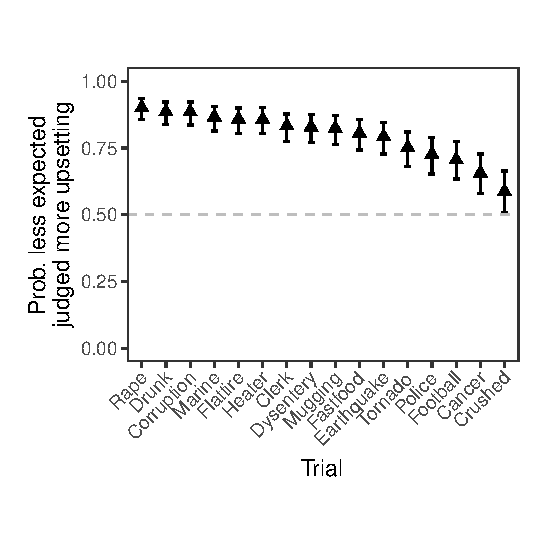
\includegraphics{fig1.eps}
\caption{Probability with which participants chose the less expected
event as more upsetting across trials in Study 1. As predicted,
participants exhibited a robust bias toward choosing the less expected
event as more upsetting across all items. Error bars represent 95\%
credible intervals calculated from the hierarchical logistic regression
model. See Supporting Information for full description of items. {}}
\end{figure}

Consistent with our predictions, manipulating expectations consistently
shaped evaluations across a range of morally-significant events. We
found that people viewed unexpected harmful events as more upsetting
than expected harmful events, even when the harm a victim suffered was
the same. For instance, people judged that a robbery at a clothing store
(unexpected) was more upsetting than a robbery at a convenience store
(expected). Furthermore, these differences were large, systematic, and
robust. Although there was variability in the situations that elicited
the largest differences, our statistical approach treated trial as a
random effect (see Methods and Results), allowing us to generalize
conclusions to items we did not test (14).

\begin{figure}
\centering
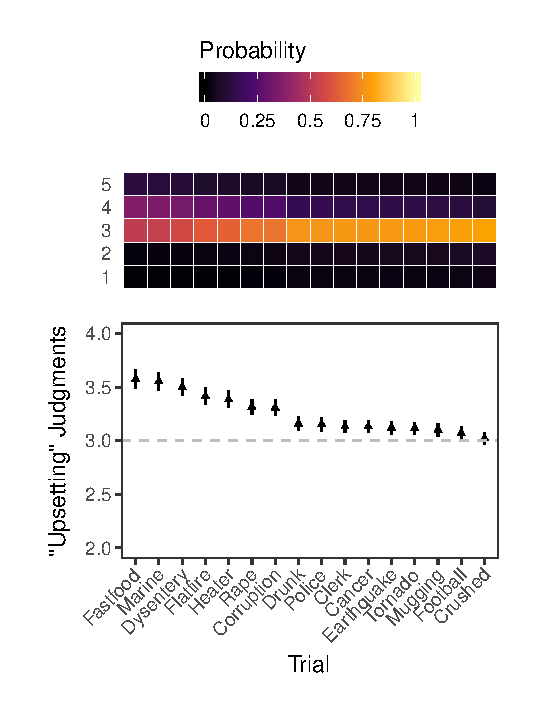
\includegraphics{fig2.eps}
\caption{Participants' responses by item in Study 2. Upper: heatmap plot
displaying probability of choosing each response on the 1 to 5 scale
across items. Lower: marginal expected response across items, with 95\%
credible interval calculated from the ordinal regression model. Note the
scale has been constrained to show relevant region of results. In both
plots, response of 3 indicates indifference, a response below 3
indicates a bias to choose the more expected event as more upsetting,
and a response above 3 indicates a bias to choose the less expected
event as more upsetting. Similar to Study 1, when participants judged
that one of the events was more upsetting, they showed a robust bias
toward choosing the less expected event as more upsetting. Trials are
sorted by response to aid readability. {}}
\end{figure}

We have argued that expectations shape our reactions to events because
they determine how informative those events are in shaping our
understanding of the world. Thus, we argue that well-grounded
information theoretic principles can account for people's divergent
moral reactions to likely and unlikely events.

There's a sense in which it is clearly adaptive that the violation of
our expectations would direct our attention to the events and situations
about which our understanding is most in need of revision. For instance,
an act of terrorism in a peaceful nation might be less expected because
of our beliefs about the effectiveness of security forces, the stability
of national relationships, and positive relationships among people
groups in that nation. Therefore, a surprising act of terrorism casts
doubt on our deeper understanding of the geopolitical situation, and
thereby leads us to suspect similar acts are more likely to occur in the
future.

Yet, however well-grounded the underlying principles, there's a clear
moral danger whenever expectations influence our moral concerns. For
instance, ``victim blaming'' describes the tendency to shift blame away
from aggressors and onto victims of crimes like sexual assault (15) and
police violence. Work by Janoff-Bulman and colleagues (16) has shown
that merely increasing the perceived probability of a victim suffering a
sexual assault induced participants to blame the victim for her assault.
People's expectations may explain the flip side of victim blaming,
whereby those who victim blame also tend to judge transgressors less
harshly: When people perceive a victims' actions as increasing the
probability of their eventual assault, they may perceive an aggressor's
actions as producing a smaller change in utility, thus warranting weaker
condemnation.

The influence of expectations on moral evaluations poses perhaps the
greatest threat when considering our reactions to humanitarian
challenges brought on by poverty or regional instability. In these
cases, the influence of expectations on moral evaluations threatens to
impose vicious and morally pernicious cycles. For instance, people
living in geo-politically unstable regions or in the developing world
are often those who are most affected by terrorism, famine, and natural
disasters, and are the very people in greatest need of assistance and
concern from the world at-large. However, for these very reasons, it is
often unsurprising when harm befalls people living in these
circumstances. Thus the influence of expectations on moral evaluations
threatens to reduce observer's concern for these victims most in need,
making people less likely to donate time or money to aid victims, or to
take political action to prevent further harms. The present research
identifies this potentially pernicious moral bias and grounds it in
information theoretic principles. Hopefully, by further understanding
these cognitive dynamics, psychologists and policymakers can begin to
find ways to reduce or counteract people's tendency to ignore the plight
of those in most need of attention.

\section*{Materials and Methods}\label{materials-and-methods}
\addcontentsline{toc}{section}{Materials and Methods}

We conducted two preregistered studies examining the role of
expectations in moral evaluations using two different judgment tasks
(\url{https://osf.io/5qnf7/}). Each study consisted of multiple trials
where participants were presented brief descriptions of two events.
Their task was to decide which of the two events was more upsetting. In
Study 1, they made a two-alternative forced-choice, and in Study 2 they
made their judgments using a five-point rating scale. Both studies
consisted of 16 experimental trials, five ``equivalent'' filler trials,
and five ``non-equivalent'' filler trials.

In experimental trials, the two events described identical harms, but
one event was more expected and one more unexpected, as determined in a
prior norming study (see SI). For example, participants considered the
following stimulus:

\begin{itemize}
\item
  ``A 30 year old man in California dies in an earthquake''
  {[}Expected{]}
\item
  ``A 30 year old man in Oklahoma dies in an earthquake''
  {[}Unexpected{]}
\end{itemize}

In each of these events, the harm to the victim is the same (death) but
one event is more probable than the other, given the different
likelihoods of earthquakes occurring in California versus Oklahoma. In
addition to being more naturalistic, manipulating expectations through
(otherwise irrelevant) contextual details helps ensure that the harm
suffered by the victim is understood to be identical. In the context of
gambles, it is possible to manipulate probabilities specifically and
directly (5). However, in the context of more realistic moral harms, any
attempt to directly manipulate probabilities risks also changing
participants' perceptions of the degree of harm. For instance, suppose
we describe two cancer patients, one with a 5\% chance of survival and
one with a 50\% chance of survival. Even if they both ultimately meet
the same fate, participants might fairly assume the patient with the
lower chance of survival had a more serious illness, was more
debilitated, suffered more severely, and so forth. In contrast, changing
the context of the two events explains away these likelihood
differences, better equating the events in other respects.

Both studies also included ``equivalent'' filler trials. In these
trials, the two events differed in trivial contextual details that we
did not expect would affect participants' judgments. These filler trials
were meant to prevent participants from becoming explicitly aware of the
structure of the experimental trials. Finally, both studies included
``non-equivalent'' filler trials, the two events differed substantially
in the degree of harm suffered by a victim, so that one event was
expected to be seen as considerably more upsetting than the other. These
trials were included to allow participants a chance to use the extremes
of the response scale and to reduce any task demands that might drive
them to make artificially fine-grained distinctions when generating
their responses. All experimental materials for these studies are
available as Supporting Information at \url{https://osf.io/5qnf7/}.

\subsection*{Exclusions}\label{exclusions}
\addcontentsline{toc}{subsection}{Exclusions}

In both studies, we excluded participants who failed to correctly answer
attention-check questions or who indicated at the end of the study they
had not taken their participation seriously.

\subsection*{Data Analysis}\label{data-analysis}
\addcontentsline{toc}{subsection}{Data Analysis}

We analyzed our data by performing Bayesian estimation using the
probabilistic programming language Stan (17). We tested our
preregistered predictions by computing Bayes Factors (i.e.~BF01) using
the hypothesis function in the R package brms. Bayes Factors express the
ratio of the probability of data under the null hypothesis to the
probability of the data under an alternative hypothesis. Larger Bayes
Factors indicate that the data are more likely under the null hypothesis
(i.e., that the intercept is not different from zero) than the
alternative hypothesis (i.e., that the intercept is different from
zero), and vice versa. As Bayes Factors can be influenced by prior
choices (Gelman, Simpson, \& Betancourt, 2017), we performed prior
robustness checks to confirm that our conclusions would not depend
substantially on the specification of the priors.

To ensure the generality of our findings, we tested participants'
reactions to a variety of items and treated both participants and items
as random effects throughout our analyses. The use of random effects
over items allows us to consider these items as a sample from a larger
population of possible items, and to generalize our findings to that
wider population, much as we generalize from our sample of participants
to the larger population (14).

\subsection*{Study 1}\label{study1}
\addcontentsline{toc}{subsection}{Study 1}

\subsubsection*{Participants}\label{s1-participants}
\addcontentsline{toc}{subsubsection}{Participants}

A total of 255 participants were recruited from Amazon's Mechanical Turk
work distribution website (mTurk). Of these, 230 passed attention checks
and were included in the final analyses (105 male, 125 female, median
age = 33 years old). All participants were paid \$0.60 for their
participation.

\subsubsection*{Materials and procedure}\label{s1-materials-procedure}
\addcontentsline{toc}{subsubsection}{Materials and procedure}

Participants judged 16 experimental event-pairs and 10 equivalent filler
event-pairs. On each trial (an example is shown above), participants
were presented with the event-pair stimulus and had to judge which
outcome was more upsetting in a two-alternative forced choice task. The
two events were labeled ``Outcome 1'' and ``Outcome 2'' and the order,
and whether Outcome 1 or 2 was the unexpected event, was randomized and
counter-balanced.

\subsubsection*{Results and discussion}\label{s1-results}
\addcontentsline{toc}{subsubsection}{Results and discussion}

We predicted that people would judge that events where unexpected harm
occurred were more upsetting than events where expected harm occurred.
As indicated in Figure 1, we observed this trend. We estimated the
magnitude of this effect by fitting a Bayesian logistic random effects
model with participants' responses as the dependent variable (1 =
unexpected event is more upsetting; 0 = expected event is more
upsetting) and random intercepts for item and subject, allowing us to
generalize both to items and subjects we did not test. The intercept in
this model represents the log-odds of selecting the unexpected event as
being more upsetting. Thus, by examining the population-level intercept,
we can test whether participants were biased toward selecting the
unexpected event (\(\beta\) \textgreater{} 0), the expected event
(\(\beta\) \textless{} 0), or were unbiased (\(\beta\) = 0). We found
that people were considerably more likely to think that unexpected
events were more upsetting than events that were expected, Intercept =
1.424, 95\% CI {[}1.147, 1.707{]}, BF01 \textless{} .001. Figure 1 shows
participants' responses broken-down by individual items. Participants'
bias toward selecting the unexpected event as more upsetting was
consistent across the 16 experimental items.

\subsection*{Study 2}\label{study2}
\addcontentsline{toc}{subsection}{Study 2}

In Study 1 we found that people's judgments of events were biased by
their expectations about those events. When forced to choose between two
events, participants decided that unexpected events were more upsetting
than expected events. In Study 2, we sought to test our hypothesis using
a more conservative method: we provided participants with a more
expressive response scale so that if they viewed the events under
consideration as equally harmful, their responses could reflect their
attitude.

\subsubsection*{Participants}\label{s2-participants}
\addcontentsline{toc}{subsubsection}{Participants}

A total of 504 participants were recruited from Amazon's Mechanical Turk
work distribution website (mTurk). Of these, 372 passed attention checks
and were included in the final analyses (174 male, 198 female, median
age = 34 years old). All participants were paid \$0.60 for their
participation.

\subsubsection*{Materials and procedure}\label{s2-materials-procedure}
\addcontentsline{toc}{subsubsection}{Materials and procedure}

The materials in Study 2 were the same as those in Study 1. As in Study
1, on each trial of the study, participants were presented with a pair
of actions labeled ``Outcome 1'' and ``Outcome 2'' and were asked,
``Which outcome seems more upsetting?'' In Study 2 participants made
their rating on a five-point scale (Outcome 1 seems more upsetting,
Outcome 1 seems a little more upsetting, neither seems more upsetting
than the other, Outcome 2 seems a little more upsetting, Outcome 2 seems
more upsetting).

\subsubsection*{Results and discussion}\label{s2-results}
\addcontentsline{toc}{subsubsection}{Results and discussion}

We predicted that participants would evaluate unexpected events as more
upsetting than expected events. We estimated the magnitude of this
effect by fitting a cumulative (ordinal) random effects model with
participants' scale responses as the dependent variable (1 to 5) and
random intercepts for item and subject. This model produces four
intercept coefficients, representing the cumulative log-odds of
responses at each scale point or lower. For instance, the second
coefficient represents the log-odds participants chose a 2 (``outcome 2
seems slightly more upsetting'') or lower on the scale. Similarly, the
third intercept coefficient represents the log-odds participants chose a
3 or lower on the scale. To examine the predicted effect, we compared
the third intercept coefficient (representing the log-odds of choosing 4
or higher) to the inverse of the second intercept coefficient (thereby
representing the log-odds \emph{not} choosing a 3 or higher--i.e.,
choosing a 1 or 2), allowing us to test whether participants were more
likely to choose the expected or unexpected event as being more
upsetting in cases where they did not choose the neither option. This
analysis indicated that people were more likely to think that events
that were unexpected were more upsetting than events that were expected,
BF01 \textless{} .001 (see supporting information for full model
results). We observed this difference consistently across nearly every
item (Figure 2).

We note that the most common response was to view both events, which
involve identical harms, as equivalently upsetting. However, when
participants did view one of the events as more upsetting, they showed a
clear bias towards choosing unexpected events as more upsetting. Thus,
Study 2 replicates the tendency to view unexpected moral events as more
upsetting using a more conservative judgment task.

\section*{Theoretical Formalization}\label{theory}
\addcontentsline{toc}{section}{Theoretical Formalization}

Evaluation (e.g., of utility) is often examined in the context of
decision-making. However, people often generate post hoc evaluations of
events for their own sake. For instance, to reflect on the results of
our choices and to evaluate others--to judge the wisdom of their
decisions or the morality of their actions.

We construe event evaluation as a comparison between the state of
affairs prior to an event and the state of affairs following the event.
We represent the state of the world as a random variable, \(X\). We
assume \(X\) is discrete, and that every realization \(x\) represents
some potential specific state of the world in all relevant aspects under
consideration. An agent has some utility function \(u\), that applies
over the different realizations of \(X\). Thus the expected utility of
the present state of the world is:

\begin{equation}
E_X[u(X)] = \sum_x u(x)p(x)
\end{equation}

When we learn an event has occurred, we can represent this as an
observation of another random variable, \(S\). We can think of \(S\) as
a ``signalling event'' because it informs (signals) to us something
about \(X\) (13). For simplicity, we treat \(S\) as binary, either 1 or
0. Importantly, we assume there is a dependency between \(S\) and \(X\),
so that observing \(S\) informs our knowledge of \(X\). For instance,
reading a news report of a terror attack in Brussels informs us about
the state of the world, telling us about what realizations of X are no
longer possible (e.g., any wherein it was a peaceful day in Brussels)
and which are more or less likely. Conditioned on \(S\), the expected
utility of the world is:

\begin{equation}
E_{X|S}[u(X)] = \sum_x u(x)p(x|s)
\end{equation}

We define the value assigned to the signalling event, \(V(S)\), as:

\begin{equation}
V(S) = E_{X|S}[u(X)] - E_X[u(X)]
\end{equation}

Which we write more specifically as:

\begin{equation}
V(s=1) = \sum_x u(x)p(x|s=1) - \sum_x u(x)p(x)
\end{equation}

Applying the expectation of conditional expectation, we can write:

\begin{equation}
V(s=1) = \sum_x u(x)p(x|s=1) - \sum_x \sum_s u(x)p(x|s)p(s)
\end{equation}

We then perform some algebra. We break out the summation over \(S\) (6),
pull the multipliers out of the last two sums (7), rewrite \(p(s=0)\) in
terms of \(p(s=1)\) (8), and factor to combine the first two sums (9).

\begin{align}
V(s=1) &= \sum_x u(x)p(x|s=1) - \sum_x u(x)p(x|s=1)p(s=1) - \sum_x u(x)p(x|s=0)p(s=0) \\
 &= \sum_x u(x)p(x|s=1) - p(s=1)\sum_x u(x)p(x|s=1) - p(s=0) \sum_x u(x)p(x|s=0) \\
 &= \sum_x u(x)p(x|s=1) - p(s=1)\sum_x u(x)p(x|s=1) - (1-p(s=1)) \sum_x u(x)p(x|s=0) \\
 &=(1-p(s=1))\sum_x u(x)p(x|s=1) - (1-p(s=1)) \sum_x u(x)p(x|s=0)
\end{align}

Finally, combining both sums by their common factor yields (10):

\begin{equation}
V(s=1)=(1-p(s=1))\sum_x u(x)p(x|s=1) - u(x)p(x|s=0)
\end{equation}

Thus, it can be seen under this formalization that the role of
expectations in the evaluation of events is fundamental--it does not,
for instance, depend on any specifics concerning the utility function
over states of the world. Instead, this conclusion depends on just two
assumptions: first, that events are evaluated by comparing the utilities
of the states of the world prior to and following the event; and second,
that knowledge of those states of the world is uncertain.

We have appealed to the informativeness of an event to illustrate
intuitively how expectations should influence evaluations. More expected
events carry less information, and thereby engender weaker reactions.
Though our model of event evaluation is not an information-theoretic
model in a direct sense, this interpretation still applies: the
information carried by observing \(S\) is a function of that
observation's prior probability, which we have in turn shown determines
its evaluation. Also relevant, although not addressed here, is the
mutual information between \(X\) and \(S\)--the extent to which \(S\)
informs \(X\).

\showmatmethods
\showacknow
\pnasbreak

\hypertarget{refs}{}
\hypertarget{ref-Trope2010}{}
1. Trope Y, Liberman N (2010) Construal-level theory of psychological
distance. \emph{Psychological review} 117(2):440--63.

\hypertarget{ref-Graham2015}{}
2. Graham DA (2015) The empathy gap between paris and beirut.

\hypertarget{ref-Greenslade2007}{}
3. Greenslade R (2007) A hierarchy of death.

\hypertarget{ref-Bell1985}{}
4. Bell D (1985) Disappointment In Decision Making Under Uncertainty.
\emph{Operations Research} 33(1):1--27.

\hypertarget{ref-Mellers1997}{}
5. Mellers B a, Schwartz a, Ho K, Ritov I (1997) Decision Affect Theory:
Emotional Reactions to the Outcomes of Risky Options.
\emph{Psychological Science} 8(6):423--429.

\hypertarget{ref-Shepperd2002}{}
6. Shepperd J a, Mcnulty JK (2002) The affective consequences of
expected and unexpected outcomes. \emph{Psychological science}
13(1):85--88.

\hypertarget{ref-Gul1991}{}
7. Gul F (1991) A theory of disappointment aversion. \emph{Econometrica}
59(3):667--686.

\hypertarget{ref-Loomes1986}{}
8. Loomes G, Sugden R (1986) Disappointment and Dynamic Consistency in
Choice under Uncertainty. \emph{Review of Economic Studies}
53(2):271--282.

\hypertarget{ref-Kahneman1979}{}
9. Kahneman D, Tversky A (1979) Prospect Theory: An Analysis of Decision
under Risk. \emph{Econometrica} 47(2):263--292.

\hypertarget{ref-Tversky1992}{}
10. Tversky A, Kahneman D (1992) Advances in prospect theory: Cumulative
representation of uncertainty. \emph{Journal of Risk and uncertainty}
5:297--323.

\hypertarget{ref-Shannon1948}{}
11. Shannon CE (1948) A Mathematical Theory of Communication. \emph{Bell
System Technical Journal} 27(3):379--423.

\hypertarget{ref-Rescorla1972}{}
12. Rescorla RA, Wagner AR (1972) A theory of Pavlovian conditioning:
Variations in the effectiveness of reinforcement and nonreinforcement.
\emph{Classical Conditioning II Current Research and Theory}, pp 64--99.

\hypertarget{ref-Arrow1996}{}
13. Arrow KJ (1996) The economics of information: An exposition.
\emph{Empirica} 23(2):119--128.

\hypertarget{ref-Judd2012}{}
14. Judd CM, Westfall J, Kenny DA (2012) Treating stimuli as a random
factor in social psychology: A new and comprehensive solution to a
pervasive but largely ignored problem. \emph{Journal of Personality and
Social Psychology} 103(1):54--69.

\hypertarget{ref-Koss2000}{}
15. Koss MP (2000) Blame, shame, and community: Justice responses to
violence against women. \emph{American Psychologist} 55(11):1332--1343.

\hypertarget{ref-Janoff-bulman1985}{}
16. Janoff-Bulman R, Timko C, Carli LL (1985) Cognitive biases in
blaming the victim. \emph{Journal of Experimental Social Psychology}
21:161--177.

\hypertarget{ref-Carpenter2017}{}
17. Carpenter B, et al. (2017) Stan : A Probabilistic Programming
Language. \emph{Journal of Statistical Software} 76(1).
doi:\href{https://doi.org/10.18637/jss.v076.i01}{10.18637/jss.v076.i01}.



% Bibliography
% \bibliography{pnas-sample}

\end{document}

